\begin{figure}[t]
% \captionsetup{font=normalsize}
% \captionsetup[sub]{font=normalsize}
\setlength{\belowcaptionskip}{0.5\baselineskip}
\centering
    \begin{subfigure}{.5\linewidth}
        \centering
        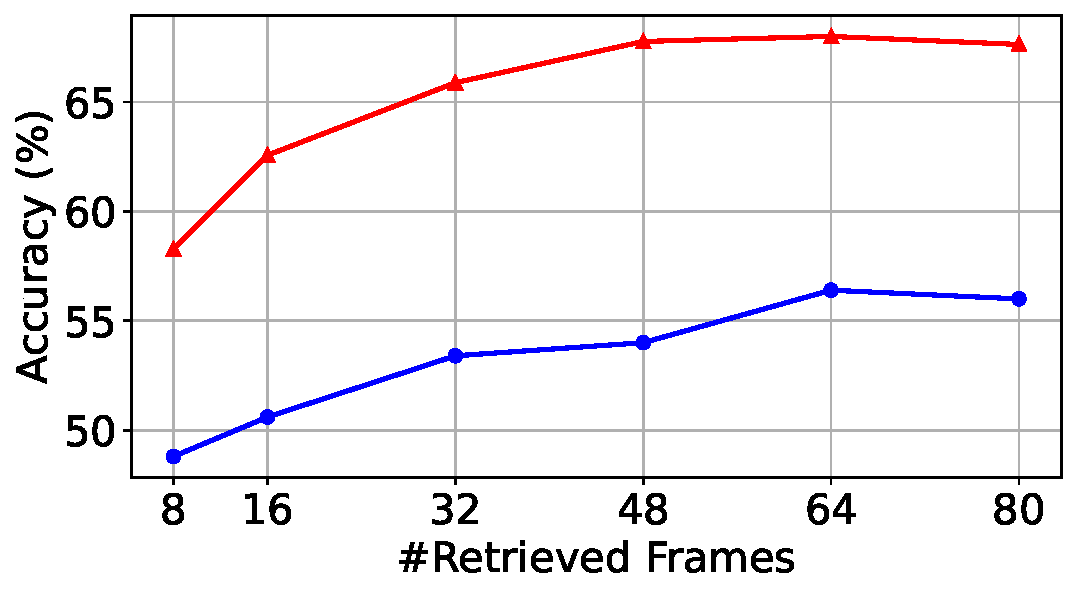
\includegraphics[width=.95\linewidth]{figures/src/retrieve_size.pdf}
        \caption{}
    \end{subfigure}%
    \hfill
    \begin{subfigure}{.5\linewidth}
        \centering
        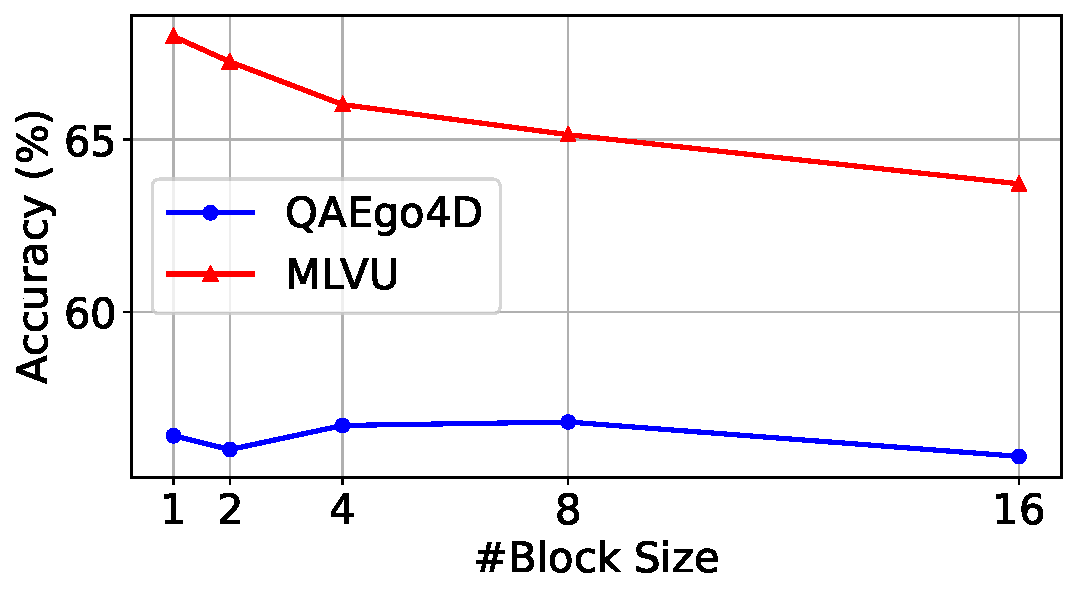
\includegraphics[width=.95\linewidth]{figures/src/chunk_size.pdf}
        \caption{}
    \end{subfigure}
\vspace{-15pt}
\caption{
\textbf{Estudio de ablación de los hiperparámetros de retrieval:}
(a) número de frames recuperados y (b) número de frames por bloque de retrieval.
Los experimentos se realizan con \texttt{LLaVA-OV-7B}.
}
\label{fig:ablation_retrieval}
\end{figure}
